% Bournemouth University PhD Thesis Template by Daniel Green (@KasumiL5x).
% 
% This template is a modification of Cambridge's PhD thesis template.
% It conforms to Bournemouth University's PhD thesis style as of 2018.
% 
% See the original README.md for information on how to use the template, including
% the variety of options available for this document class.
\documentclass[a4paper,12pt,customfont,custommargin,custombib,oneside,draft,PageStyleI]{PhDThesisPSnPDF}
% [draft] Draft mode (line numbers, watermarks)
% [print] Turns off colored links and possibly some other features that paper cannot do.
% [oneside] Single-sided (combine with print turned off).
% [twoside] Double-sided (combine with print turned on; chapters start on left page and add blank pages to allow this).
% 
% Final online version:
% \documentclass[a4paper,12pt,customfont,custommargin,custombib,oneside,PageStyleI]{PhDThesisPSnPDF}
% 
% Final print version:
% \documentclass[a4paper,12pt,customfont,custommargin,custombib,twoside,PageStyleI]{PhDThesisPSnPDF}


% ****************************** Preamble ******************************
% Contains packages, user-defined commands, and settings.
% ****************************** Packages, Commands, Settings ******************************

% ****************************** Custom Margin ******************************
% Use the document class option 'custommargin' to use this section.
% Set {innerside, outerside, top, bottom} and other page dimensions.
\ifsetCustomMargin
  \RequirePackage[left=40mm,right=25mm,top=35mm,bottom=30mm]{geometry}
  \setFancyHdr % To apply fancy header after geometry package is loaded.
\fi




% ****************************** Paragaph Spacing ******************************
% Add spaces between paragaphs.
% \setlength{\parskip}{0.5em}

% Enabling ragged bottom avoids extra whitespaces between paragraphs.
\raggedbottom

% Use this to remove excess top spacing for enumerations, lists, and descriptions.
% \usepackage{enumitem}
% \setlist[enumerate,itemize,description]{topsep=0em}




% ****************************** Line Spacing ******************************
% Pick the linespacing that suits your university guidelines.  Default is one-half line spacing.
% \doublespacing
% \onehalfspacing
% \singlespacing




% ****************************** Custom Fonts ******************************
% Use the document class option 'customfont' to use this section.  If you don't,a default LaTeX font will be used.
\ifsetCustomFont
  % For example:
  % 
  % \RequirePackage{helvet}
  % For use with XeLaTeX.
  % \setmainfont[
  %   Path           = ./libertine/opentype/,
  %   Extension      = .otf,
  %   UprightFont    = LinLibertine_R,
  %   BoldFont       = LinLibertine_RZ, % Linux Libertine O Regular Semibold
  %   ItalicFont     = LinLibertine_RI,
  %   BoldItalicFont = LinLibertine_RZI, % Linux Libertine O Regular Semibold Italic
  % ]
  % {libertine}
  % Load font from system font.
  % \newfontfamily\libertinesystemfont{Linux Libertine O}
\fi




% ****************************** Custom Packages ******************************
% Here you can add your own custom packages and configure them.  The ones listed are common suggestions.

% \usepackage{algpseudocode} % Algorithms and pseudocode (https://ctan.org/pkg/algorithmicx).

\RequirePackage[labelsep=space,tableposition=top]{caption} % Customize float captions (https://ctan.org/pkg/caption).
\renewcommand{\figurename}{Fig.} % To support older versions of captions.sty.

% \usepackage{rotating} % Rotation of figures and tables (https://ctan.org/pkg/rotating).
% \usepackage{wrapfig} % Wrap text around figures and tables (https://ctan.org/pkg/wrapfig).
\usepackage{subcaption} % Multiple captions within a figure (https://ctan.org/pkg/subcaption).
\usepackage{booktabs} % Professional looking tables (https://ctan.org/pkg/booktabs).
\usepackage{multirow} % Table cells that can span multiple rows (https://ctan.org/pkg/multirow).
% \usepackage{multicol} % Table cells that can span multiple columns (https://ctan.org/pkg/multicol).
% \usepackage{longtable} % Tables that can spread over multiple pages (https://ctan.org/pkg/longtable).
% \usepackage{tabularx} % Extends tabular to include paragraph-like column expansion; tabulary also exists (https://ctan.org/pkg/tabularx).
% \usepackage{float} % Makes placing figures and tables easier.  In particular, [H] for exact placement (https://ctan.org/pkg/float).
% \restylefloat{figure} % If you use the float package, enable this.

\usepackage{siunitx} % Ability to use SI unit symbols (https://ctan.org/pkg/siunitx).

% \usepackage[perpage]{footmisc} % Customizable footnote options (https://ctan.org/pkg/footmisc).




% ****************************** Enumeration Breaking ******************************
% Set boundaries to stop enumations (etc.) from breaking across pages in an ugly way (defaults to 10000).
% \clubpenalty=500
% \widowpenalty=500




% ****************************** References ******************************
% Packages and settings relating to referencing.

% \usepackage{cleveref} % Automatic referencing without explicitly stating fig/table (https://ctan.org/pkg/cleveref).

% Use the document class option 'custombib' to use this section.
\ifuseCustomBib
   \RequirePackage[square, sort, numbers, authoryear]{natbib} % Provide your custom bib package here.  In this case, natbib.
% If you would like to use biblatex for your reference management, as opposed to the default `natbibpackage` pass the option `custombib` in the document class. Comment out the previous line to make sure you don't load the natbib package. Uncomment the following lines and specify the location of references.bib file.
% \RequirePackage[backend=biber, style=numeric-comp, citestyle=numeric, sorting=nty, natbib=true]{biblatex}
% \bibliography{references/references} %Location of references.bib only for biblatex
\fi

% Changes the default 'Bibliography' name into 'References'.
\renewcommand{\bibname}{References}




% ****************************** Custom Commands ******************************
% Custom commands can be defined and configured here.

% For changing the name of ToC, LoF, LoT.
% \renewcommand{\contentsname}{My Table of Contents}
% \renewcommand{\listfigurename}{My List of Figures}
% \renewcommand{\listtablename}{My List of Tables}

% ToC depth and section numbering depth.
\setcounter{secnumdepth}{2}
\setcounter{tocdepth}{2}

% Changes the name of the nomenclature section.
% \renewcommand{\nomname}{Symbols}

% The default value of \appendixtocname and \appendixpagename is 'Appendices'.  These commands can change that.
% \renewcommand{\appendixtocname}{List of appendices}
% \renewcommand{\appendixname}{Appndx}




% ****************************** Draft Mode Settings ******************************
% Sets up options for draft mode (enable by using the draft option).

% Uncomment to disable figures in draft mode.
% \setkeys{Gin}{draft=true}  % Set draft to false to enable figures in draft mode.

% Set the watermark text.
% \SetDraftText{DRAFT}

% Set the watermark location.  Can use 'top' or 'bottom'.
% \SetDraftWMPosition{bottom}

% Set the version number for the draft.  Defaults to v1.0.
% \SetDraftVersion{v1.1}

% Draft text grayscale value (where 0 is black and 1 is white).  Defaults to 0.75.
% \SetDraftGrayScale{0.8}




% ****************************** Todo Notes Settings ******************************
% Uncomment the following lines to enable todonotes.
% \ifsetDraft
% 	\usepackage[colorinlistoftodos]{todonotes}
% 	\newcommand{\mynote}[1]{\todo[author=kks32,size=\small,inline,color=green!40]{#1}}
% \else
% 	\newcommand{\mynote}[1]{}
% 	\newcommand{\listoftodos}{}
% \fi

% Example todo: \mynote{Enter your note text here.}



% ****************************** Thesis Info ******************************
% Various bits of information for the thesis, mostly relating to frontmatter.
% ****************************** Thesis Information & Metadata ******************************

% Title of the thesis.
\title{Title}
% Subtitle (optional).
\subtitle{Subtitle}


% Author's name.
\author{Your Name}


% Department.
\dept{Department of Science and Technology}
% University name.
\university{Bournemouth University}


% Short university logo.  Minimum 30mm.  If you use this, do not use the long logo.
% \crest{
\includegraphics[width=0.3\textwidth]{logos/bu_logo_short}}
% Long university logo.  Minimum 65mm.  If you are using this, do not use the short logo.
\crest{
\includegraphics[width=0.65\textwidth]{logos/bu_logo_long}}
% Shield logo.  Minimum 30mm.  This is not required, but can make the titlepage look nicer.
\collegeshield{
\includegraphics[width=0.2\textwidth]{logos/bu_logo_short}}


% Supervisor (optional).  For multiple supervisors, append using \newline command.
\supervisor{Dr. S. Supervisor}
% Role of supervisors.  Defaults to 'Supervisor'.  Can be left blank for no role.
% \supervisorrole{\textbf{Supervisors: }}
% Line width for supervisors.  Play with this to align multiple supervisors if you have to.
%\supervisorlinewidth{0.35\textwidth}

% Advisor (optional).  For multiple advisors, append using \newline command
%\advisor{Dr. A. Advisor}
% Role of advisors.  Defaults to 'Advisor'.  Can be left blank for no role.
% \advisorrole{Advisors: }
% Line width for advisors.  Play with this to align multiple advisors if you have to.
%\advisorlinewidth{0.25\textwidth}


% Submission text before the title of the degree.
\renewcommand{\submissiontext}{A thesis submitted in partial fulfillment of the requirements for the degree of}
% Full title of the awarded degree.
\degreetitle{Doctor of Philosophy}


% Affiliation (optional).
% \college{Affiliation Here}


% Submission date.  Defaults to {\monthname[\the\month]\space\the\year}.
%\degreedate{October 2017}


% Metadata about the thesis.
\subject{Interactive Narrative}
\keywords{
	{Authoring}
	{Games}
	{Narrative}
	{PhD Thesis}
	{Science and Technology}
	{Bournemouth University}
}



% ****************************** Abstract Only ******************************
% If using the 'abstract' document class option, only the titlepage and abstract will print out.
% This section lets you include what is printed when this option is enabled.
\ifdefineAbstract%
 \pagestyle{empty}
 \includeonly{front/declaration, front/abstract}
\fi


% ****************************** Chapters Only ******************************
% If using the 'chapter' document class option, only specific chapters and references are printed.
% This section lets you include what is printed when this option is enabled.
\ifdefineChapter%
 \includeonly{chapters/compiling/compiling}
\fi


\begin{document}


% ****************************** Front Matter ******************************
% Everything before your actual work begins. This follows Bournemouth's suggestion (which is not fixed).
\frontmatter
\maketitle
% !TEX root = ../thesis.tex

% ****************************** University Copyright ******************************

\begin{unicopyright}
\textit{This copy of the thesis has been supplied on condition that anyone who consults it is understood to recognise that its copyright rests with its author and due acknowledgement must always be made of the use of any material contained in, or derived from, this thesis.}
\end{unicopyright}
 % Required by Bournemouth to come instantly after the titlepage.
% !TEX root = ../thesis.tex

% ****************************** Thesis Abstract ******************************

% Don't forget you can use the 'abstract' option to print only the titlepage and abstract.

\begin{abstract}
The abstract should be approximately 300 words and should give a synopsis of the thesis stating the nature and scope of the work undertaken and of the contribution made to the knowledge of the subject treated. It should appear on its own as a single page (and should be headed by the author's full name and the title of the thesis, but nobody seems to do this).
\end{abstract}

\tableofcontents
\listoffigures
\listoftables
% !TEX root = ../thesis.tex

% ****************************** Thesis Acknowledgements ******************************

\begin{acknowledgements}
The acknowledgement should include reasons for undertaking the study as well as acknowledgement of assistance, for example, support such as scholarships and grants, consultations and discussions with Supervisory Team and colleagues.\\
And I would like to acknowledge\dots
\end{acknowledgements}

% !TEX root = ../thesis.tex

% ****************************** Thesis Declaration ******************************

\begin{declaration}
Bournemouth's instructions for a PhD thesis declaration are:

\textit{The author should draw attention to any material contained in the thesis that has been presented before. If the thesis is based on joint research, the nature and extent of the author's individual contribution should be stated. The declaration should follow the acknowledgement, under a separate heading.}

There is no standard declaration available, so feel free to find one online and tailor it to your own requirements, providing you meet the above statement.

% Author and date will be inserted automatically from thesis.tex \author \degreedate.
\end{declaration}

\printnomenclature% You can add spacing between symbols and descriptions using [3em] etc.
% ****************************** Thesis Dedidcation ******************************

\begin{dedication} 
I would like to dedicate this thesis to\dots
\end{dedication}



% ****************************** Main Matter ******************************
% This is where your actual work starts. \mainmatter sets everything up.
\mainmatter%

% This is where you put your chapters. I split my chapters into files for organization. Below, they are included in the document.
% Notice how you don't need the file extension!
% !TEX root = ../../thesis.tex

% I recommend having a separate 'main file' for each chapter.
% In this case, the 'Introduction' chapter lives in [chapters/introduction/introduction.tex].
\chapter{Introduction}%

% This command sets a name that we can later refer to (e.g., See Chapter~\ref{ch:introduction}).
% It's a good idea to have them, but they aren't required.
% While not required at all, here are my own personal rules for naming labels:
% All label names are in the format `category:name`.
% The `name` portion should be a hierarchy from the chapter down through sections if sections are labeled too to the element.
%  They should be separated by hyphens to allow for underscores in individual names. (e.g., ch-sec-fig_name).
% The `category` portion should be a category as follows:
% 	 Chapter: ch
% 	 Section: sec
% Subsection: subsec
% 	Appendix: appdx
% 	   Table: table
% 	  Figure: fig
\label{ch:introduction}%

% This sets the root folder for your graphics for THIS chapter. In this case, [chapters/introduction/figures].
% It stops bloating of a single 'figures' folder and helps to separate them out.
\graphicspath{{chapters/introduction/figures/}}

Welcome! Here is a brief description of what \LaTeX{} is.

\LaTeX{} is a document preparation system for the \TeX{} typesetting program.
It offers programmable desktop publishing features and extensive facilities for automating most aspects of typesetting and desktop publishing, including numbering and cross-referencing, tables and figures, page layout, bibliographies, and much more.
\LaTeX{} was originally written in 1984 by Leslie Lamport and has become the dominant method for using \TeX{}; few people write in plain \TeX{} anymore.
The current version is \LaTeXe{}.

The remainder of this document will briefly expose you to the basics of \LaTeX{}.

% !TEX root = ../../thesis.tex

\chapter{The Uber Basics of \LaTeX{}}%
\label{ch:basics}%
\graphicspath{{chapters/basics/figures/}}

This chapter will briefly expose you to the basics.
It is not a replacement for looking things up online, so make sure you do that too.
I particularly like \url{https://www.overleaf.com/learn} as it is quite digestible.
Make sure you're reading through the actual source files at the same time, as I have left practical comments explaining in more detail than you see here.

I recommend you start by opening \verb|thesis.tex| which is the main file of this template.
Take note of the \verb|\documentclass| command at the top which provides many options for how your document looks.
By default, this template is setup for one-sided A4 paper, 12pt font, a custom font, custom margins, a custom bibliography style, a specific type of heading on each page, and has draft mode turned on (which is why you see line numbers in the margins and a watermark in the footer).
I have included the configurations that I used for my online and print thesis submission variations.

% My personal structure is to have a 'main' file for each chapter, in this case `basics.tex', which then
% includes several other files, one for each section (we will get to structure later on).
% I recommend this method as once your thesis becomes large, having monolithic files can be difficult to manage.

% This is how you directly paste a file into another file.
% ! IMPORTANT NOTE !
% See how this is `input` rather than `include` in thesis.tex? There's an extremely important difference.
% Using `include` will ensure the included content starts on a NEW page. That is, if you're one line over a page and use `include`, it will skip the rest of that page entirely.
% Using `input` will treat it as if you just copy and pasted the file's contents here, not skipping anything.
% !TEX root = ../../thesis.tex

\section{Structure}%
\label{sec:basics-structure}%

\LaTeX{} can organize and number your document automatically with several sectioning commands.
From the highest to the lowest, the commands are:

\begin{itemize}[noitemsep,left=1pt]
  \item \verb|\part{name}|
  \item \verb|\chapter{name}|
  \item \verb|\section{name}|
  \item \verb|\subsection{name}|
  \item \verb|\subsubsection{name}|
  \item \verb|\paragraph{name}|
  \item \verb|\subparagraph{name}|
\end{itemize}

\noindent In your thesis, you are likely to only use \verb|\chapter|, \verb|\section|, \verb|\subsection|, and \verb|\subsubsection|.
The file \verb|basics.tex| defines a chapter, which is represented above by ``Chapter 2''.
This file, \verb|structure.tex|, defines a section, which is represented above as ``2.1''.
When we add subsections, they would be represented as ``2.1.1'' and so on.

The style of these sectioning commands has been customized for this thesis. Look for ``Custom Titles'' in \verb|preamble.tex| for more information.

\subsection*{Unnumbered Sectioning}%
This subsection is not listed in the table of contents and doesn't have a number.
You can achieve this with any of the sectioning commands by appending them with an asterisk.

% !TEX root = ../../thesis.tex

\section{Formatting}%
\label{sec:basics-formatting}%

Formatting text in \LaTeX{} is easy, for the most part.
You can make text \textbf{bold} by wrapping it in \verb|\textbf{}|.
You can make text \textit{italic} by wrapping it in \verb|\textit{}|.
You can \underline{underline} text by wrapping it in \verb|\underline{}|.
These can of course be \textbf{\textit{\underline{combined}}} together.

It is important to be aware that \verb|\textit{}| and \verb|\emph{}| almost always act similar, but in fact do different things in different contexts.
In short, \verb|\emph{}| behaves differently as you nest it in different commands, and some packages may in fact change its behavior.
If you want something that's \textit{definitely} italic, stick with \verb|\textit{}|.

This thesis template also uses the \texttt{soul} package which extends the formatting options you have available.
For example, we can \st{strike through} text by wrapping it in \verb|\st{}|.

It is also worth noting that many special characters in \LaTeX{} have reserved meanings, so you cannot use them verbatim.
Consider, for example, the ampersand (\&), percent (\%), and dollar (\$) symbols.
These characters must be \textit{escaped} by placing a backslash (\textbackslash) before them.
In this case, we would write \verb|\&|, \verb|\%|, and \verb|\$|.

\subsection{Quotes}%
You should \textbf{never} use double quotes directly within \LaTeX{} to wrap quoted text.
Instead, you should insert backticks to the left of the quote, and apostrophes to the right (see \verb|formatting.tex|).
These can both stack indefinitely, so add them to your heart's content!

For example, ``this quote has two backticks before it and two apostrophes after it'' whereas `this quote only has one either side'.
We can also display block quotes as follows:

\begin{displayquote}[][]
  ``This block of text is displayed centered on the page and represents a chonkier block of text than you'd typically quote inline. Here is some more filler text to make this quote much longer. Significantly longer. In fact, so long that I'm not quite sure what to add here other than these padding words.'' 
\end{displayquote}

\subsection{Lists}%
Use the \verb|enumerate| environment to list things by number.

\begin{enumerate}[noitemsep,topsep=0pt]
  \item Items within enumerate blocks are numbered automatically.
  \item By default, this starts at 1, but it can be configured with the \texttt{enumitem} package.
  \item There's no limit to the length of these, as long as they are one line.
\end{enumerate}

\vspace{5pt}

\noindent Use the \verb|itemize| environment to list arbitrary things by bullet point.

\begin{itemize}[noitemsep,topsep=0pt]
  \item This is an example bullet point.
  \item So is this one.
  \item And this one!
\end{itemize}

\vspace{5pt}

\noindent You can use the \verb|description| environment to list items with descriptions, although I usually tend to do this by hand.

\begin{description}[noitemsep,topsep=0pt]
  \item[The Title] A short description that follows.
  \item[Another Title] This can be any length, as long as it's one line.
\end{description}

\vspace{5pt}

\noindent These environments can be nested and configured quite deeply, so do look them up!

\subsection{Footnotes}%
You can add footnotes to any text by using the \verb|\footnote{}| command.
Do \textbf{not} add a space before the command as a superscript number will be inserted in its place.

By default, this thesis template will place all footnotes at the \textbf{end} of the document, delineated by which chapter they appear in.
This is a personal preference and some people prefer to see them on the same page at the bottom.
I dislike having them on the same page as they can begin to take up some serious space and introduce formatting oddities, whereas when they are at the end of the document, their length and quantity really doesn't matter.
Look at \verb|preamble.tex| for more information on how to toggle between these two modes.

Here are several examples of footnotes.
Popular search engines include Google\footnote{Available at \url{https://www.google.com}.}, Bing\footnote{Available at \url{https://www.bing.com}.}, and DuckDuckGo\footnote{Available at \url{https://duckduckgo.com}.}.
Also note that this template includes a custom \verb|\AsOfToday| command that you can use to automatically specify `today' when building your document.
It is helpful for specifying when a link was last valid, for example\footnote{Imagine I'm talking about an amazing website available at \url{www.website.com} \AsOfToday.}.

% !TEX root = ../../thesis.tex

\section{Figures \& Tables}%
\label{sec:basics-figures_and_tables}%

\subsection*{Figures}%
Figures are typically made up of a \verb|figure| environment, a \verb|\centering| command to keep the content aligned in the middle of the page, an \verb|\includegraphics| command to insert the image itself, a \verb|\caption| command to insert a caption, and a \verb|\label| command to give it a referenceable name, which we will look at later.

Figure~\ref{fig:basics-skyrim_book} shows how to insert a single figure with a caption.
The image is inserted using the \verb|\includegraphics| command, where its \verb|width| option is used to size the image relative to the text's maximum width.
A caption is also added and placed below the image with the \verb|\caption| command, and \verb|\label| is used to provide an anchor that we can reference in text, as the start of this paragraph did.
The position of the image is controlled by both its literal position in the \LaTeX{} source as well as an optional argument to the \verb|\figure| environment.
Placement of figures in \LaTeX{} can be tricky and they can often end up where you don't want them to!

% Note how this is wrapped in the 'figure' environment. The "!htbp" is a positioning hint. Have a search online for more details.
\begin{figure}[!htbp]
  % This ensures that the image is centered on the page. You almost always want this.
  \centering
  % This is now we include graphics. The argument in the square brackets defines the image width as a 0-1 percentage of the text's width.
  % You can also use direct sizes here, too, but this is most common. The actual image is specified WITHOUT its extension.
  % Remember in the parent basics.tex file, we set graphics path as "\graphicspath{{chapters/basics/figures/}}"?
  % The images are relative to that. As other chapters refined graphicspath, they become relative to that path, and so on.
  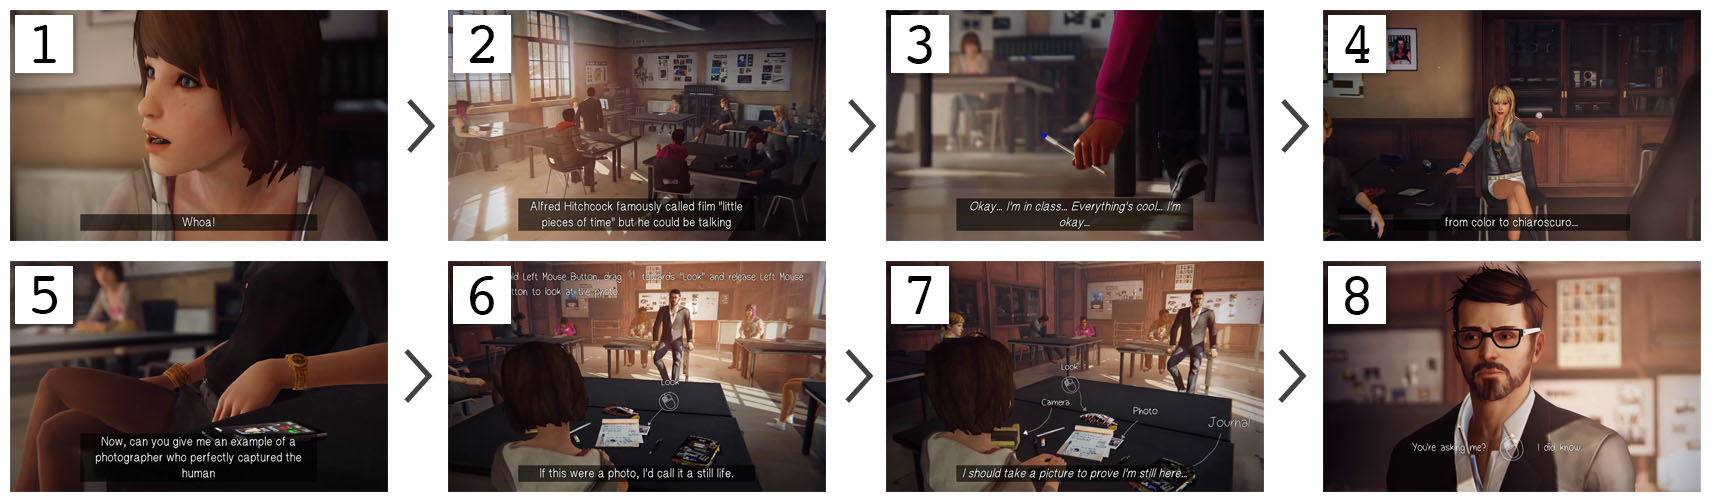
\includegraphics[width=1.0\textwidth]{lis-overview}
  % This caption appears below the image. If you want it above, simply move the line up above \includegraphics.
  \caption{A high-level overview of the \textit{Life is Strange} sequence. 1.\ Max wakes up in class. 2.\ A lecture is taking place. 3.\ Stella drops her pen. 4.\ Taylor bullies Kate. 5.\ Victoria's phone vibrates. 6.\ Max's desk interactions. 7.\ Max's camera usage prompt. 8.\ Max's questioning for disturbing class.}%
  % This defines a label that we can \ref{} later, which we will be doing!
  \label{fig:basics-skyrim_book}
\end{figure}

Figure~\ref{fig:basics-obra} shows how to stack multiple images together in one figure either horizontally or vertically.
We can even reference its parts like Figure~\ref{fig:basics-obra_1} and Figure~\ref{fig:basics-obra_2}.
In this template, this is achieved with the \verb|subfig| package and its \verb|\subfloat| command.

% Notice how there are TWO labels here. This lets us reference Figure X.A, X.B separately.
\begin{figure}[!htbp]
  \centering
  
  % Notice how we're using the \subfloat command to insert a caption, then \includegraphics and \label are used inside its brackets.
  \subfloat[Entering Part 4 of Chapter IV by interacting with Bun-Lan Lin's body. Parts 1, 2, and 3 unavailable at this point.]{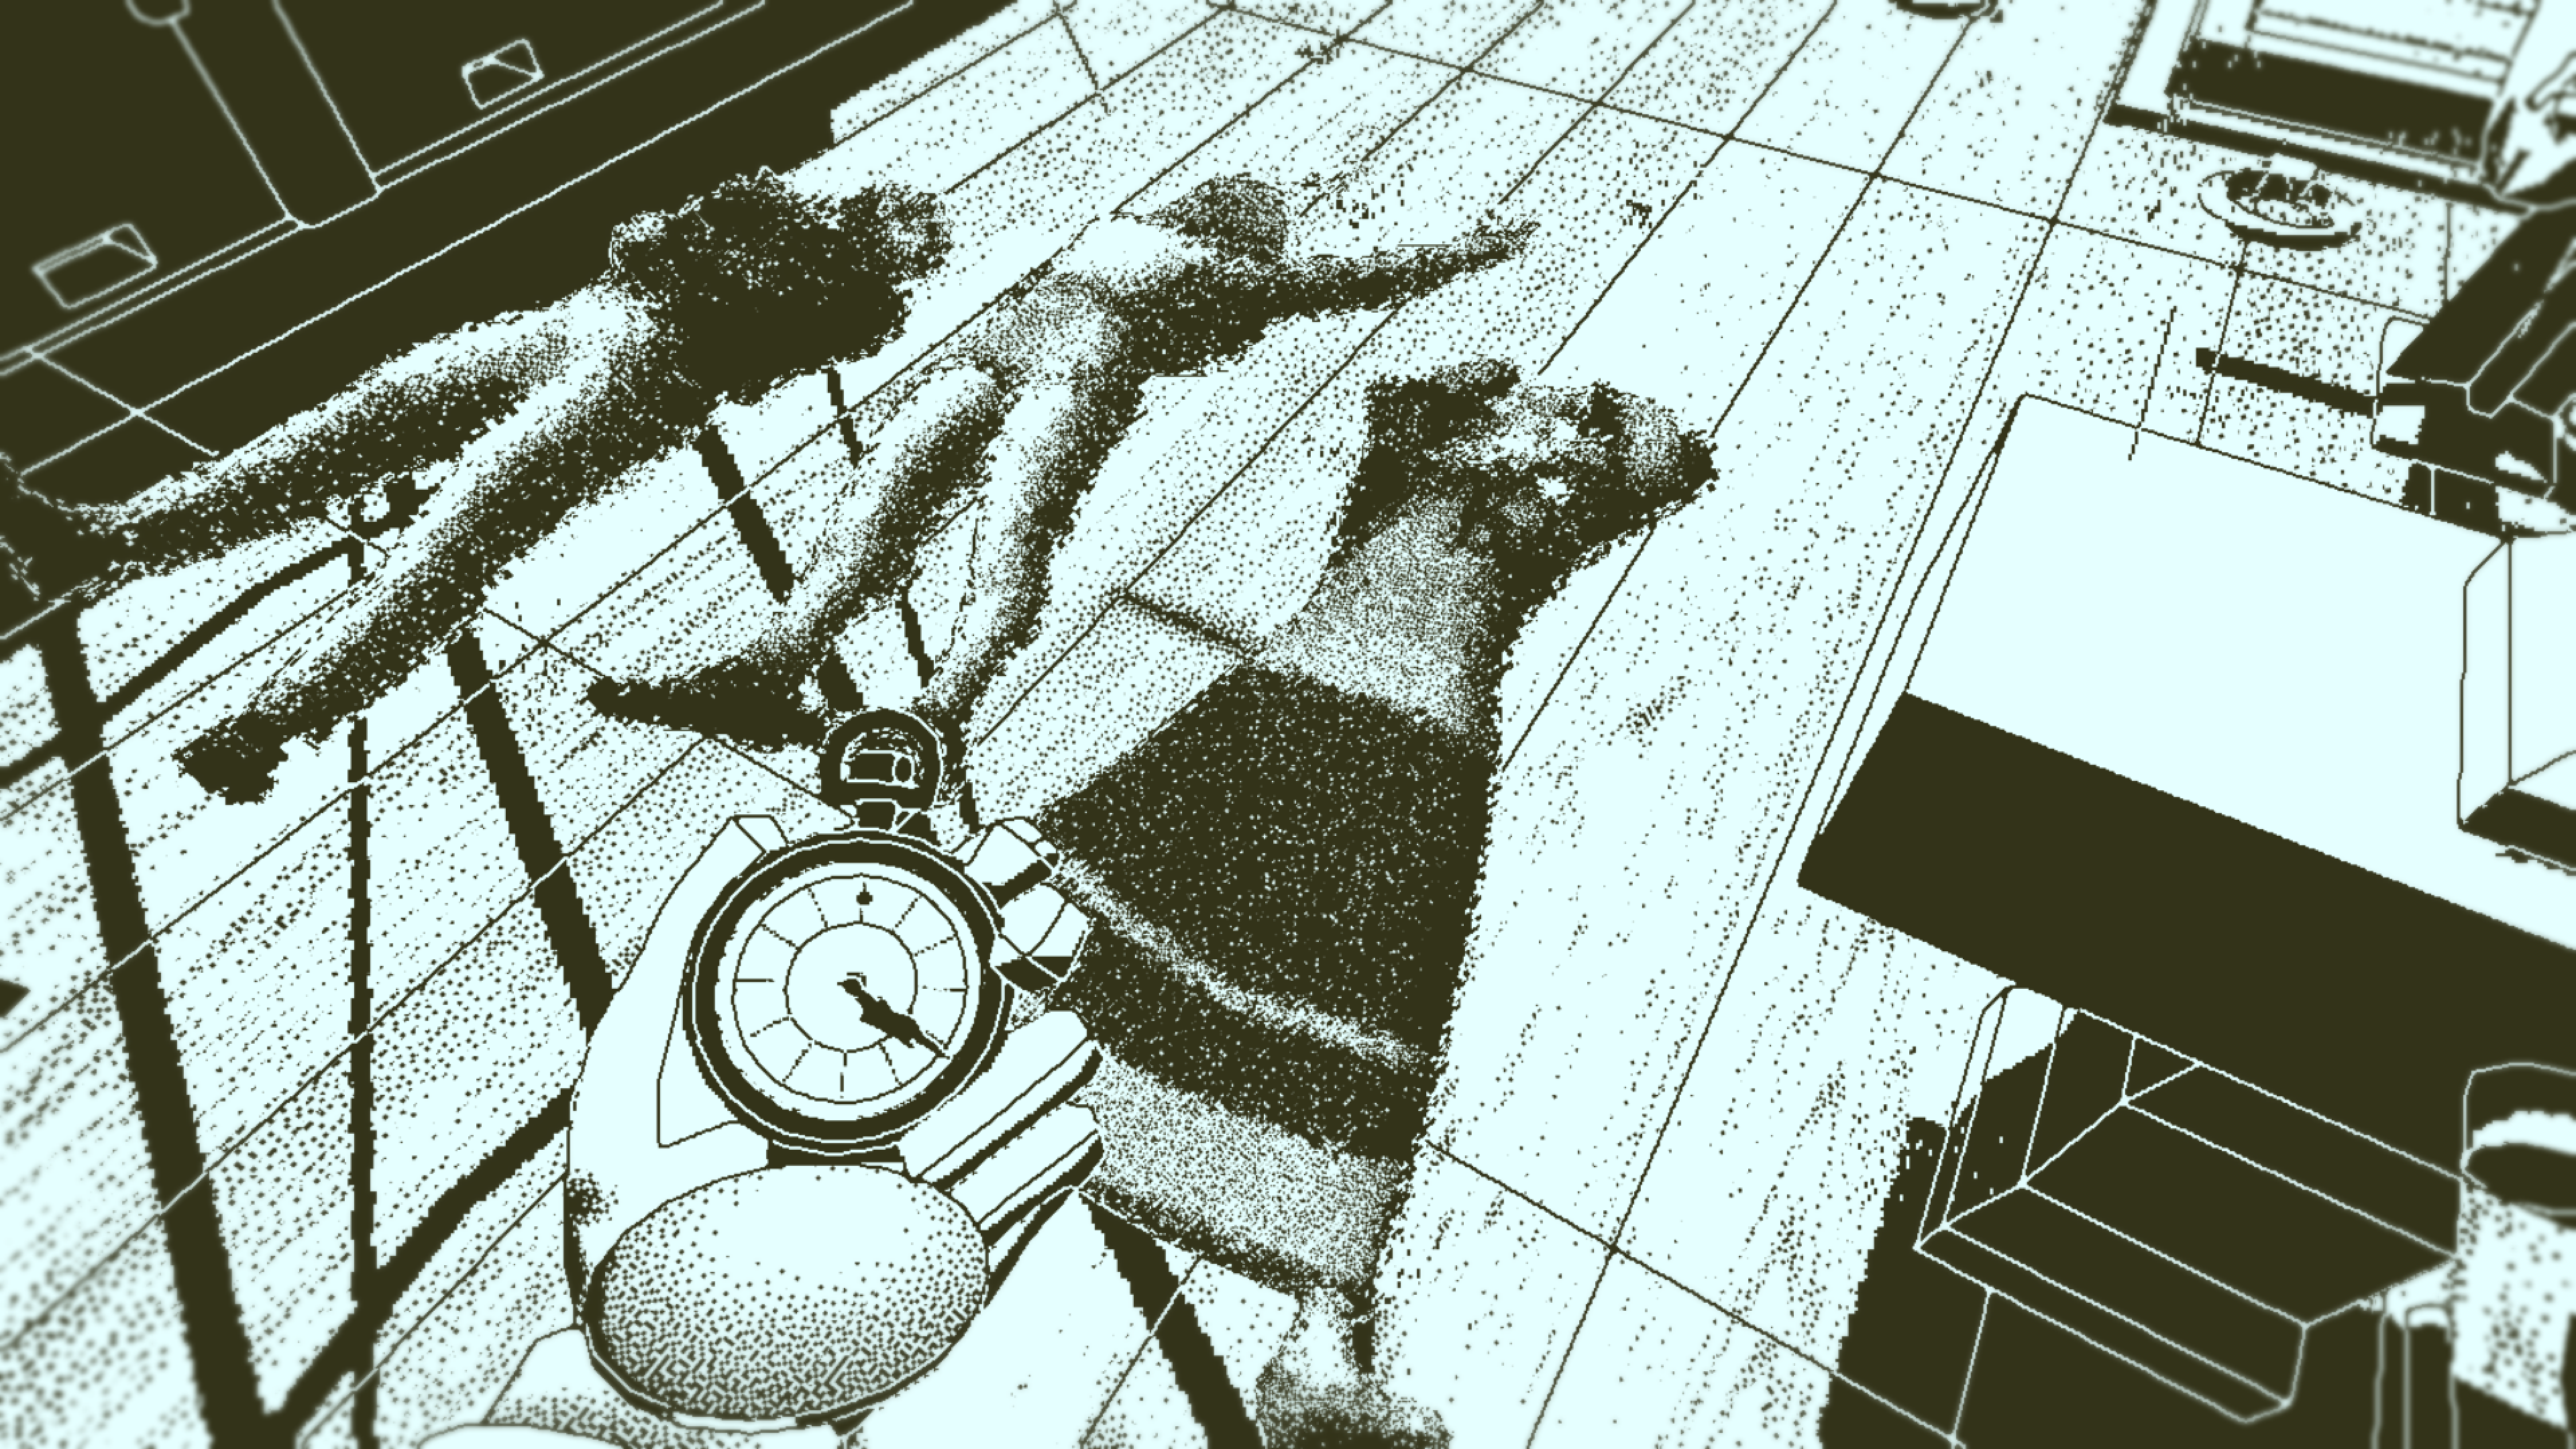
\includegraphics[width=.48\textwidth]{obra-1}\label{fig:basics-obra_1}}
  % This helps with spacing between horizontal images.
  \quad
  % Notice how the size is less than 50% (0.48 in this case). This is so that there's room around each image for spacing.
  % If you just used 50%, they would stack vertically instead of horizontally.
  \subfloat[Entering Part 2 from within Part 4 by locating and interacting with Patrick O'Hagan's body.]{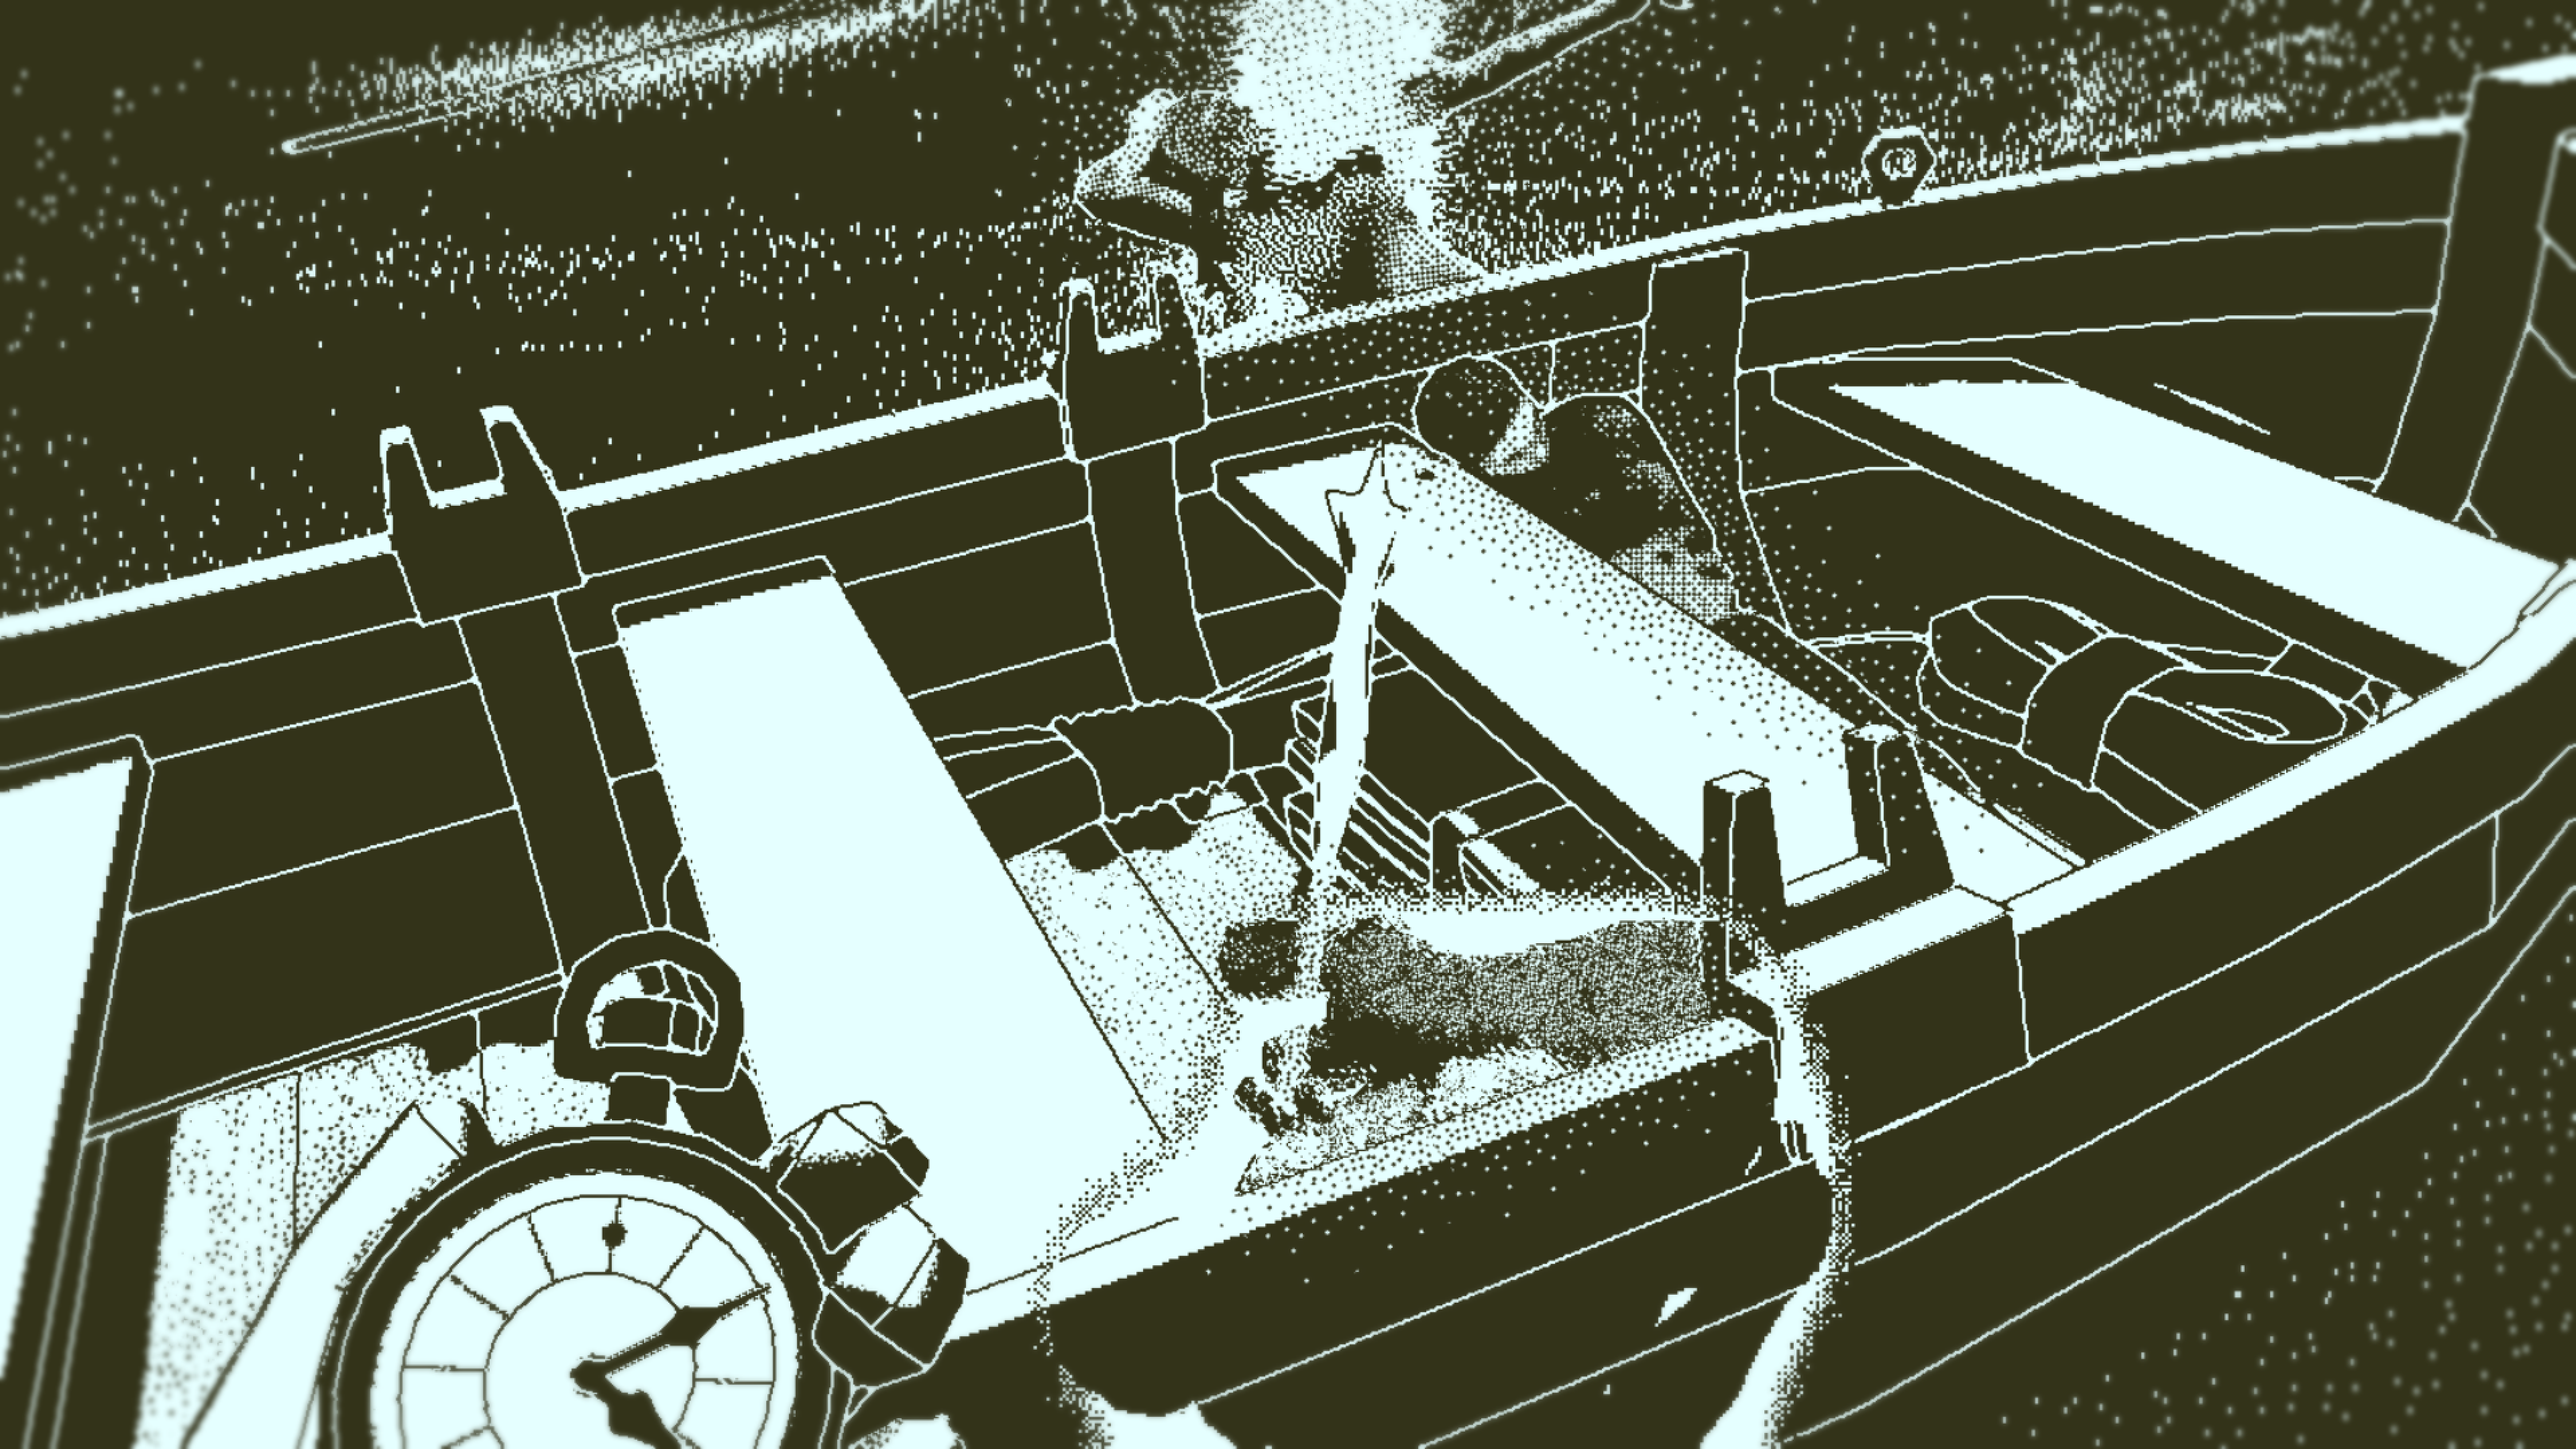
\includegraphics[width=.48\textwidth]{obra-2}\label{fig:basics-obra_2}}
  \caption{A player in \textit{Return of the Obra Dinn} entering into Part 4 of Chapter IV by interacting with Bun-Lan Lin's body on the main deck. From Part 4, they discover Patrick O'Hagan's body, which can take them to Part 2 of the same Chapter.}

  \label{fig:basics-obra}
\end{figure}

\subsection*{Tables}%
Tables can be a nightmare in \LaTeX{}, but once working, can give very elegant results.
I strongly recommend you look up how to create effective tables online.
This thesis template already comes with several packages that enhance or otherwise improve tables.

You should always wrap your tables in the \verb|table| environment if you want them to have captions and be referenceable.

Table~\ref{table:basics-table_1} shows a relatively complex table.
Check out the \LaTeX{} source for more details which explains how everything works.
Tables often look best at the \textbf{top} of a page, but here they are forced to be nearby.

% This is just like {figure} but with a table inside. Captions and labels are *typically* at the top of a table.
\begin{table}[!htbp]
  \centering
  \caption{A relatively complex table with multi-column headings, skipped headings, automatic width columns, and more.}%
  \label{table:basics-table_1}
  
  % If you want your tables to be smaller (or larger), you can insert this (or another size) INSIDE the table environment.
  % \footnotesize

  % The first parameter specifies the overall width of the table.
  % The second complex looking parameters determine the columns and their sizes/behaviors.
  \begin{tabularx}{\linewidth}{>{\raggedright\arraybackslash}p{0.63\linewidth} *3{X} | *3{X}}
    % This is the top row. Notice how there's an empty &. This skips the first column.
    % The multicolumn{3} commands merge 3 cells into one piece of text.
    & \multicolumn{3}{c}{Topic A} & \multicolumn{3}{c}{Topic B}\\
    % This is the second line of the heading which doesn't skip any columns.
    Summarizing Title & A & B & C & A & B & C\\
    % This adds a full width line to segment the header from the rest of the table.
    \toprule
    
    % Here are the table entries. Notice how all but the last one end in \\. This is how you start a new row.
    Mauris porttitor, arcu id sagittis & 10 & 0 & 12 & 6 & 0 & 7\\
    Nullam erat mauris, consectetur nec & 0 & 8 & 0 & 0 & 5 & 0\\
    Integer elementum lobortis ligula vitae & 7 & 2 & 0 & 7 & 2 & 0\\
    Maecenas id magna in neque & 1 & 1 & 5 & 1 & 1 & 5\\
    Curabitur tincidunt est vel magna & 0 & 5 & 2 & 0 & 5 & 2
    \end{tabularx}
\end{table}

Table~\ref{table:basics-discoverable_narrative_table} show below has a much more complex setup with custom colors and nested multiline cells.
In this table, there are no headings at the top, but instead the left column has been used.
Each cell to the right of the headings column has a title and a subtitle within it.
Typically, adding line breaks into a cell is challenging and can introduce formatting troubles.
This table uses the \verb|makecell| package to create custom cells with line breaks in them which \LaTeX{} treats as a single cell.

\definecolor{DNHeaderColor}{HTML}{568eae}
\definecolor{DNRowColor1}{HTML}{ffffff}
\definecolor{DNRowColor2}{HTML}{f5f6f8}
\newcommand{\DNCell}[1]{\Gape[2pt][2pt]{#1}} % Arguments to Gape are vertical spacing around the cell up then down.
\newcommand{\DNHeaderCol}{\color{white}\cellcolor{DNHeaderColor}}
\newcommand{\DNRowColOne}{\cellcolor{DNRowColor1}}
\newcommand{\DNRowColTwo}{\cellcolor{DNRowColor2}}
\begin{table}[!htbp]
  \centering
  \caption{\textit{Discoverable Narrative's} four-dimensional descriptor consisting of \textit{Tangibility}, \textit{Functionality}, \textit{Clarity}, and \textit{Delivery}.}%
  \label{table:basics-discoverable_narrative_table}

  \sffamily % Only for this scope.
  \begin{tabularx}{\linewidth}{r l X}
    \DNHeaderCol\textbf{Tangibility} &
    \DNRowColOne\DNCell{\makecell[l]{Tangible\\{\footnotesize Attached to an in-game object.}}} &
    \DNRowColOne\makecell[l]{Intangible\\{\footnotesize \textbf{Not} attached to an in-game object.}}\\

    \DNHeaderCol\textbf{Functionality} &
    \DNRowColTwo\DNCell{\makecell[l]{Narrative\\{\footnotesize Primary purpose is for narrative.}}} &
    \DNRowColTwo\makecell[l]{Mechanical\\{\footnotesize Primary purpose is \textbf{not} for narrative.}}\\

    \DNHeaderCol\textbf{Clarity} &
    \DNRowColOne\DNCell{\makecell[l]{Explicit\\{\footnotesize Clearly and well defined.}}} &
    \DNRowColOne\makecell[l]{Implicit\\{\footnotesize Abstract and interpretative.}}\\

    \DNHeaderCol\textbf{Delivery} &
    \DNRowColTwo\DNCell{\makecell[l]{Active\\{\footnotesize Requires interaction.}}} &
    \DNRowColTwo\makecell[l]{Passive\\{\footnotesize Is observed or experienced.}}\\
  \end{tabularx}
\end{table}

For more advanced tables that spread across multiple pages, you should check out the included \verb|xltabular| package.

% !TEX root = ../../thesis.tex

\section{Citing \& Referencing}%
\label{sec:basics-citing_and_referencing}%

\subsection*{Citing External Works}%
When citing external works, you must firstly add an entry to a \verb|.bib| file.
This template includes \verb|mypubs.bib| for your own works and \verb|\references.bib| for other works.
Once you have added an entry to a \verb|.bib| file, you are ready to cite it in text.

By default, this template uses a custom bibliography style named \verb|ieeecustom| which derives from the original \verb|ieee| style.
The only modification is that it uses \textit{Sentence Case Like This} rather than \textit{Regular case like this}.
Feel free to change this in \verb|preamble.tex|.

\begin{table}[!htbp]
  \centering
  \caption{A list of the most common citation commands.}%
  \label{table:basics-citing_examples}
  
  \begin{tabular}{>{\raggedright\arraybackslash}p{0.55\linewidth} >{\raggedright\arraybackslash}p{0.35\linewidth}}
    \textbf{Command} & \textbf{Example}\\
    \toprule

    \verb+Example~\cite{green_useoftools_2021}+ & Example~\cite{green_useoftools_2021}\\
    \verb+\citeauthor*{green_useoftools_2021}+ & \citeauthor*{green_useoftools_2021}\\
    \verb+\citeauthor{green_useoftools_2021}+ & \citeauthor{green_useoftools_2021}\\
    \verb+\citeyear{green_useoftools_2021}+ & \citeyear{green_useoftools_2021}

    \end{tabular}
\end{table}

Table~\ref{table:basics-citing_examples} shows several of the most common citation commands and an example of each.
Take careful note of the \verb|~| symbol before \verb|\cite|.
This character is a \textit{non-breaking space} which means that the word before it, in the above case ``Example'', will not be separated from the text that follows, in the above case the \verb|\cite| command.
Practically, this means that you will never have a word and its citation separate from one another at a line break, for instance.
It is important to note that \verb|~| \textbf{replaces} a regular space between the two, but visually appears identical; only its behavior changes.

It is also possible insert a complete citation by using the \verb|\fullcite| command:

\medskip

\noindent\fullcite{green_useoftools_2021}


\subsection*{Citing Internal Elements}%
If you instead want to reference something \textbf{internal} to the document, such as a figure, table, or chapter and so on, then you will be using the \verb|\ref| command.

If you look back at the tables, figures, and section headings in the \LaTeX{} code so far, you'll see liberal use of the \verb|\label| command.
This is what creates an anchor that we can use \verb|\ref| to refer to.

I may want to raise something discussed in Chapter~\ref{ch:introduction}, or a specific section such as \S\ref{sec:basics-formatting}.
Tables and figures are exactly the same --- consider Table~\ref{table:basics-citing_examples} or Figure~\ref{fig:basics-skyrim_book}.

Again note the use of \verb|~| as a non-breaking space before \verb|\ref|.
The exception to this is when using the \verb|\S| command (\S), as that symbol typically does not have a space at all.

% !TEX root = ../../thesis.tex

\section{Other Tips}%
\label{sec:basics-other}%

\subsection{Dummy Text / Lipsum}%
If you're blocking out structure and want some filler text, you can use the \verb|\lipsum| command.
Make sure to look up the package documentation on ctan\footnote{\url{https://www.ctan.org/pkg/lipsum}} as it's very flexible.

\lipsum[4]


\subsection{Code Snippets}%
This template uses the \verb|listings| package for inserting code snippets both inline and as blocks/figures.
Again, check the documentation on ctan, which I recommend any time you have questions about a package.

\begin{lstlisting}[language=c++, numbers=left, caption={Checking if a number is even using bit magic.}]
bool isEven( const unsigned int uValue ) {
  return (uValue & (uValue - 1)) == 0;
}
\end{lstlisting}

An alternative package to try is \verb|minted| which you may prefer over \verb|listings|.
It is not included in this template, so you will have to include it manually.


\subsection{Local Environment}%
I do not recommend using Overleaf for your thesis, but instead recommend setting up a local development environment.
This is because you are likely to hit the compilation time limit on Overleaf at some point late in your thesis, and switching environments last second could be a significant disturbance.
Moreover, in my own thesis I've used several advanced features or packages that outright crash Overleaf.
On the flip side, I do recommend having a blank version of this template on Overleaf so that you can quickly play around with formatting (such as building a complex table) and get instant feedback on errors and visuals.

To get \LaTeX{} on your machine, you can visit the main \LaTeX{} download page at \url{https://www.latex-project.org/get} and choose your operating system appropriately.
Personally, I use MiKTeX\footnote{\url{https://miktex.org}} on Windows and MacTeX\footnote{\url{https://www.tug.org/mactex}} on Mac.

To actually write \LaTeX{}, I use \textit{Visual Studio Code} with several helpful plugins.
I recommend using \textit{Better Comments} (colored comments to help make notes easier to find), \textit{LaTeX Workshop} (for mature LaTeX support), and \textit{Todo Tree} (to make ``TODO:'' comments stand out and findable in a list).


\subsection{Version Control}%
I recommend that you store your thesis in some kind of version control such as git.
You will inevitably want to go back and see previous versions of your document, and this is a great way of doing so.

You may have noticed looking through these documents that I have a \textbf{single} sentence per line.
This is intentional.
If you have a gigantic paragraph per line and you change even a single character, the entire line becomes modified, which makes detecting what changed quite hard.
If you instead have a line per sentence, then this makes it easier to find changes as they happen.

\subsection{Nomenclature}
Nomenclature lets you define a glossary of terms at the start of your document.
See the \LaTeX{} source here for how to define them.
Note that seeing changes to nomenclature requires building an index.
See \S\ref{ch:compiling} for more details.

% See the `nomencl' package documentation for details (https://www.ctan.org/pkg/nomencl).
\nomenclature[z-ALU]{ALU}{Arithmetic Logic Unit}
\nomenclature[z-BEM]{BEM}{Boundary Element Method}
\nomenclature[z-CFD]{CFD}{Computational Fluid Dynamics}
\nomenclature[z-CK]{CK}{Carman - Kozeny}
\nomenclature[z-DEM]{DEM}{Discrete Element Method}
\nomenclature[z-FEM]{FEM}{Finite Element Method}
\nomenclature[z-FLOP]{FLOP}{Floating Point Operations}
\nomenclature[z-FPU]{FPU}{Floating Point Unit}
\nomenclature[z-FVM]{FVM}{Finite Volume Method}
\nomenclature[z-GPU]{GPU}{Graphics Processing Unit}
\nomenclature[z-LBM]{LBM}{Lattice Boltzmann Method}
\nomenclature[z-LES]{LES}{Large Eddy Simulation}
\nomenclature[z-MPM]{MPM}{Material Point Method}
\nomenclature[z-MRT]{MRT}{Multi-Relaxation Time}
\nomenclature[z-PCI]{PCI}{Peripheral Component Interconnect}
\nomenclature[z-PFEM]{PFEM}{Particle Finite Element Method}
\nomenclature[z-RVE]{RVE}{Representative Elemental Volume}
\nomenclature[z-SH]{SH}{Savage Hutter}
\nomenclature[z-SM]{SM}{Streaming Multiprocessors}


% !TEX root = ../../thesis.tex

\chapter{Compiling Your Thesis}%
\label{ch:compiling}%

% NEW CHAPTER:
% Getting started with this document.
%   - Deleting everything and starting fresh.
%   - Compiling with the bat/sh files.

Several shell/batch scripts are included in the root folder to aid in compiling your thesis.
They all internally use the \textbf{latexmk} build tool.
You can open the files for more details.\\

\noindent You can run \textbf{build-final.sh/.bat} to completely rebuild your thesis from scratch.
This will clean your project folder of temporary files, build the project once, build the index for nomenclature, and build the project again.
The result is a PDF that's guaranteed to be the latest reflection of your \LaTeX{} code, but it is the slowest approach.\\

\noindent If you have already compiled your thesis and want to see iterative changes, like changing the body of the document, and you don't care about rebuilding the nomenclature, you can use \textbf{build-once.sh/.bat}.
Note that this does not recreate your PDF from scratch, so it is faster.
However, if you suspect that your changes are not being reflected in the PDF, then try the above \textbf{build-final.sh/.bat} script instead.\\

\noindent The \textbf{build-fresh.sh/.bat} script is the same as \textbf{build-once.sh/.bat}, but it instructs \textbf{latexmk} to always process all files even if they didn't change.\\

\noindent The \textbf{build-clean.sh/.bat} script tells \textbf{latexmk} to clean all temporary files that it creates during compilation.
You can use this to clean up your project directory, but it will require a full rebuild next time.\\

\noindent If you already have a build of your thesis and want to manually rebuild the index for nomenclature, you can use \textbf{build-index.sh/.bat}.
Note that you'll need to rebuild again after this to see the changes in the PDF.\\

\noindent There is also a legacy \textbf{compile-thesis.sh/.bat} script you can look at which uses \textbf{pdflatex} directly.



% ****************************** Back Matter ******************************
% This should remain commented out if you are using appendices after your references.
% \backmatter


% ****************************** Bibliography ******************************
% This is where your references are configured and printed.
\begin{spacing}{0.9}
  % An optional line break fix here instead of in preamble as it can apparently break formatting (https://tex.stackexchange.com/a/172000).
  \setlength{\emergencystretch}{1em}%
  \printbibliography[heading=bibintoc, title={References}]

  % Alternatively, if not using a custom bib. Choose one bibliographystyle.
  % \bibliographystyle{apalike} % [1] etc.
  % \bibliographystyle{unsrt} % Use for unsorted references.
  % \bibliographystyle{plainnat} % Use this to have URLs listed in references.
  % \cleardoublepage
  % \bibliography{references/references} % Path to your References.bib file.
\end{spacing}


% ****************************** Appendices ******************************
% Your extra appendices following references are listed here.
\begin{appendices}
% !TEX root = ../thesis.tex

% ****************************** Thesis Appendix A ******************************
\chapter{How to install \LaTeX}

\section*{Windows OS}

\subsection*{TeXLive package - full version}
\begin{enumerate}
\item	Download the TeXLive ISO (2.2GB) from\\
\href{https://www.tug.org/texlive/}{https://www.tug.org/texlive/}
\item	Download WinCDEmu (if you don't have a virtual drive) from \\
\href{http://wincdemu.sysprogs.org/download/}
{http://wincdemu.sysprogs.org/download/}
\item	To install Windows CD Emulator follow the instructions at\\
\href{http://wincdemu.sysprogs.org/tutorials/install/}
{http://wincdemu.sysprogs.org/tutorials/install/}
\item	Right click the iso and mount it using the WinCDEmu as shown in \\
\href{http://wincdemu.sysprogs.org/tutorials/mount/}{
http://wincdemu.sysprogs.org/tutorials/mount/}
\item	Open your virtual drive and run setup.pl
\end{enumerate}

or

\subsection*{Basic MikTeX - \TeX~ distribution}
\begin{enumerate}
\item	Download Basic-MiK\TeX (32bit or 64bit) from\\
\href{http://miktex.org/download}{http://miktex.org/download}
\item	Run the installer
\item	To add a new package go to Start >> All Programs >> MikTex >> Maintenance (Admin) and choose Package Manager
\item	Select or search for packages to install
\end{enumerate}

\subsection*{TexStudio - \TeX~ editor}
\begin{enumerate}
\item	Download TexStudio from\\
\href{http://texstudio.sourceforge.net/\#downloads}
{http://texstudio.sourceforge.net/\#downloads}
\item	Run the installer
\end{enumerate}

\section*{Mac OS X}
\subsection*{MacTeX - \TeX~ distribution}
\begin{enumerate}
\item	Download the file from\\
\href{https://www.tug.org/mactex/}{https://www.tug.org/mactex/}
\item	Extract and double click to run the installer. It does the entire configuration, sit back and relax.
\end{enumerate}

\subsection*{TexStudio - \TeX~ editor}
\begin{enumerate}
\item	Download TexStudio from\\
\href{http://texstudio.sourceforge.net/\#downloads}
{http://texstudio.sourceforge.net/\#downloads}
\item	Extract and Start
\end{enumerate}


\section*{Unix/Linux}
\subsection*{TeXLive - \TeX~ distribution}
\subsubsection*{Getting the distribution:}
\begin{enumerate}
\item	TexLive can be downloaded from\\
\href{http://www.tug.org/texlive/acquire-netinstall.html}
{http://www.tug.org/texlive/acquire-netinstall.html}.
\item	TexLive is provided by most operating system you can use (rpm,apt-get or yum) to get TexLive distributions
\end{enumerate}

\subsubsection*{Installation}
\begin{enumerate}
\item	Mount the ISO file in the mnt directory
\begin{verbatim}
mount -t iso9660 -o ro,loop,noauto /your/texlive####.iso /mnt
\end{verbatim}

\item	Install wget on your OS (use rpm, apt-get or yum install)
\item	Run the installer script install-tl.
\begin{verbatim}
	cd /your/download/directory
	./install-tl
\end{verbatim}
\item	Enter command `i' for installation

\item	Post-Installation configuration:\\
\href{http://www.tug.org/texlive/doc/texlive-en/texlive-en.html\#x1-320003.4.1}
{http://www.tug.org/texlive/doc/texlive-en/texlive-en.html\#x1-320003.4.1}
\item	Set the path for the directory of TexLive binaries in your .bashrc file
\end{enumerate}

\subsubsection*{For 32bit OS}
For Bourne-compatible shells such as bash, and using Intel x86 GNU/Linux and a default directory setup as an example, the file to edit might be \begin{verbatim}
edit $~/.bashrc file and add following lines
PATH=/usr/local/texlive/2011/bin/i386-linux:$PATH;
export PATH
MANPATH=/usr/local/texlive/2011/texmf/doc/man:$MANPATH;
export MANPATH
INFOPATH=/usr/local/texlive/2011/texmf/doc/info:$INFOPATH;
export INFOPATH
\end{verbatim}
\subsubsection*{For 64bit OS}
\begin{verbatim}
edit $~/.bashrc file and add following lines
PATH=/usr/local/texlive/2011/bin/x86_64-linux:$PATH;
export PATH
MANPATH=/usr/local/texlive/2011/texmf/doc/man:$MANPATH;
export MANPATH
INFOPATH=/usr/local/texlive/2011/texmf/doc/info:$INFOPATH;
export INFOPATH

\end{verbatim}



%\subsection{Installing directly using Linux packages}
\subsubsection*{Fedora/RedHat/CentOS:}
\begin{verbatim}
sudo yum install texlive
sudo yum install psutils
\end{verbatim}


\subsubsection*{SUSE:}
\begin{verbatim}
sudo zypper install texlive
\end{verbatim}


\subsubsection*{Debian/Ubuntu:}
\begin{verbatim}
sudo apt-get install texlive texlive-latex-extra
sudo apt-get install psutils
\end{verbatim}

\end{appendices}

% ****************************** Footnotes ******************************
% Comment this out if you don't have footnotes at the end (see preamble.tex).
\printendnotes%


% ****************************** Index ******************************
% If you have an index, print it here.
\printthesisindex%

\end{document}
